\section{Описание манипулятора}\label{part_description_of_robot}
Рассматриваемый в данной работе манипулятор робота Kuka Youbot представляет собой пятизвенный манипулятор, снабженный двухпальцевым схватом.
Описание его массогабаритных параметров дается таблицей~\ref{table_gen_info_of_manipulator} и рисунком~\ref{img:sizes_of_robot}.
Неуказанные там параметры робота, требуемые для дальнейших расчетов, неизвестны и поэтому подлежат измерению или идентификации, речь о которых пойдет ниже по тексту.

\begin{table}[h!]
	\caption{Общая информация о манипуляторе робота Kuka Youbot.}
	\begin{center}
		\begin{tabular}{|l|c|}
			\hline
			\multicolumn{1}{|c|}{Параметр} & \makebox[3cm]{Значение}\\
			\hline
			Количество сочленений & 5\\
			\hline
			Масса & 5.3~кг\\
			\hline
			Допустимая нагрузка & $0.5$~кг\\
			\hline
			Точность повторного воспроизведения позиции & 1~мм\\
			\hline
			Максимальная скорость в сочленении & $90^\circ\text{ с}^{-1}$\\
			\hline
			Интерфейс & EtherCAT\\
			\hline
			Напряжение питание & 24~В\\
			\hline
		\end{tabular}
	\end{center}
	\label{table_gen_info_of_manipulator}
\end{table}


\begin{figure}[p]
    \center{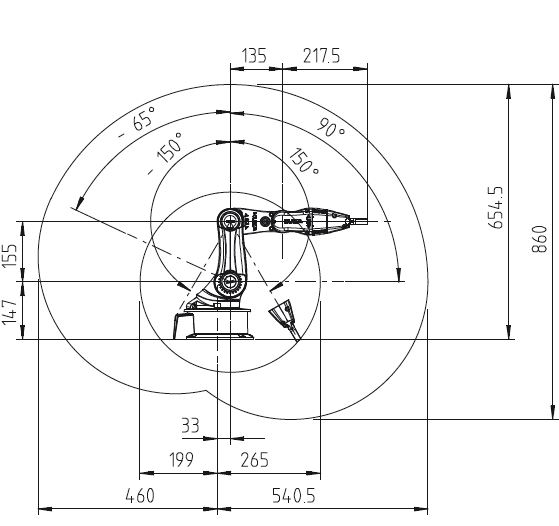
\includegraphics[width=0.7\textwidth]{youbot_workspace_1.jpg} \\ а)}
    \vfill
	\begin{minipage}[h]{0.47\linewidth}
		\centering{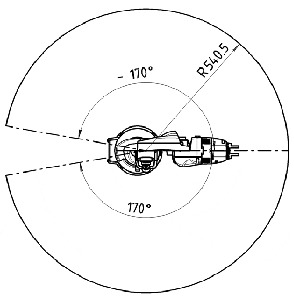
\includegraphics[width=0.95\linewidth]{youbot_workspace_2.jpg} \\ б)}
	\end{minipage}
	\hfill
	\begin{minipage}[h]{0.47\linewidth}
		\centering{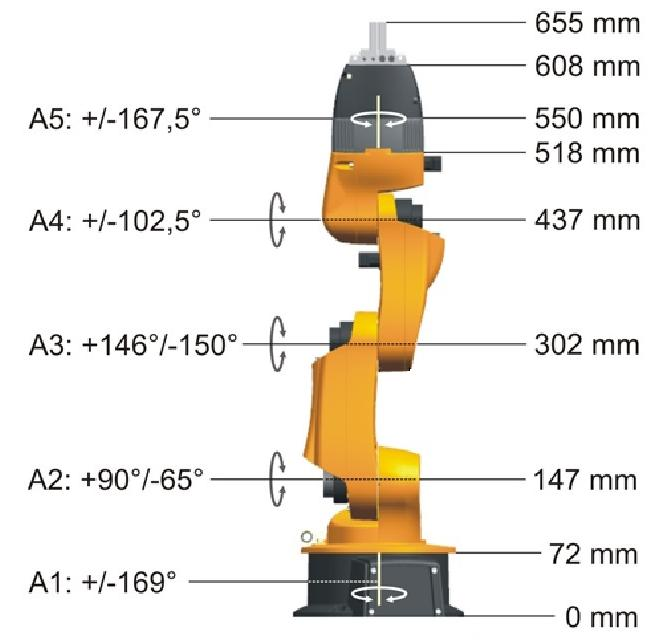
\includegraphics[width=0.95\linewidth]{youbot_length.jpg} \\ в)}
	\end{minipage}
	\caption{Некоторые параметры манипулятора Kuka Youbot: a~--- размеры рабочей области; б~--- размеры рабочей области (вид сверху); в~--- длины звеньев и предельные значения для углов вращения по каждому из сочленений~\cite{youbot_detailed_specifications}.}
	\label{img:sizes_of_robot}
\end{figure}

\newpage